\section{Resultados}
\label{sec:resultados}

\subsection{Perfil de la cohorte y calidad del registro}
\label{sec:4.1}

El corte del 24 de julio de 2026 reúne 62.043 niños y 13.884.056 mediciones. El seguimiento, sin embargo, no está completo para todos: aproximadamente el 78 \% de los niños con registro inicial llega al control de 40 semanas y el 46 \% al de 12 meses. En la revisión exploratoria encontramos 33 fechas imposibles, 985 episodios registrados antes del nacimiento y once variables cuyos rangos coincidían con los extremos observados, por lo que no resultaban útiles como control de calidad. También observamos que el redondeo del peso a 100 g pasó del 0,9 \% al 5,4 \% tras el cambio de sistema de 2022. Estos hallazgos ayudaron a definir cómo preparar y evaluar los datos.

La Figura~\ref{fig:3} muestra cómo cambia la cobertura de peso a lo largo de las visitas. Tener una medición registrada no significa necesariamente que el niño haya asistido a todos los controles. Además, cuando la información disminuye con el tiempo, los resultados obtenidos solo con los casos completos pueden dejar de representar a toda la población inicial.

\begin{figure}[t]
\centering
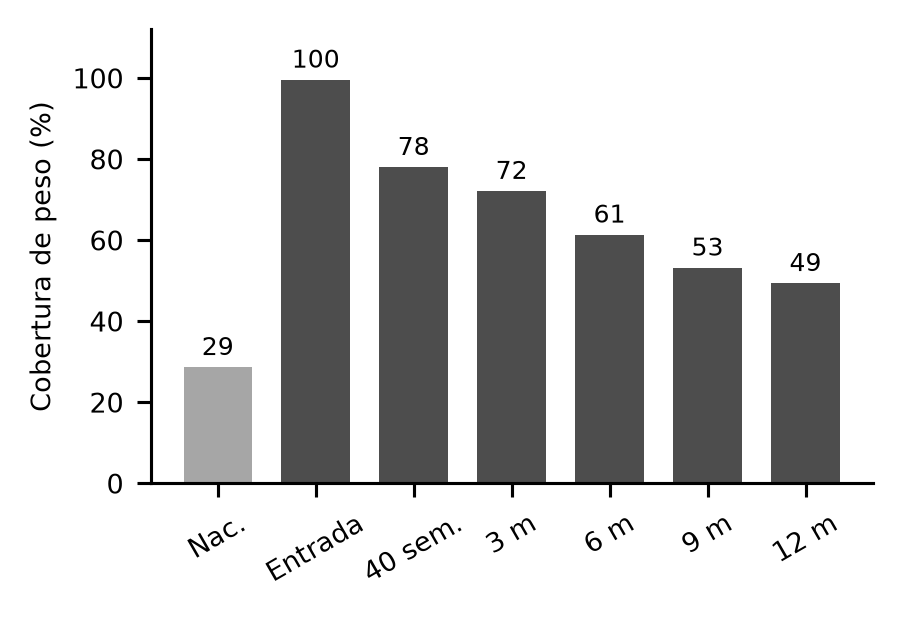
\includegraphics[width=\columnwidth]{figuras/image3.png}
\caption{Cobertura del peso por visita entre niños elegibles (corte del 24/07/2026). Elaboración propia.}
\label{fig:3}
\end{figure}

\subsection{Desempeño del detector de anomalías}
\label{sec:4.2}

Evaluamos el modelo de anomalías que está en producción (versión 7, $\alpha$ = 0,05) con los datos del corte del 24 de julio de 2026. El detector entrenó 132 modelos contextuales en 9,9 minutos. Identificó el 83,6 \% de los errores introducidos para la prueba y emitió 65,1 alertas por cada 1.000 registros limpios, frente a 14,7 de las reglas de rangos. Como muestra la Figura~\ref{fig:4}, mejoró la detección de desviaciones de tres DE (90 \% frente a 25 \%) y de etapas intercambiadas (77 \% frente a 6 \%). Los valores tomados de otro niño siguieron siendo los más difíciles de detectar (53 \%). El umbral $\alpha$ regula el equilibrio entre detectar y alertar: con $\alpha$ = 0,005, el mismo modelo detecta el 75,6 \% de los errores con 18,9 alertas por cada 1.000 registros limpios.

Estos resultados son útiles para comparar métodos, pero no representan el porcentaje de errores reales que el sistema encontraría en una clínica. Para saber cuántas alertas corresponden a problemas verdaderos hace falta la revisión de los profesionales, preferiblemente sin mostrarles previamente la predicción del modelo.

\begin{figure}[t]
\centering
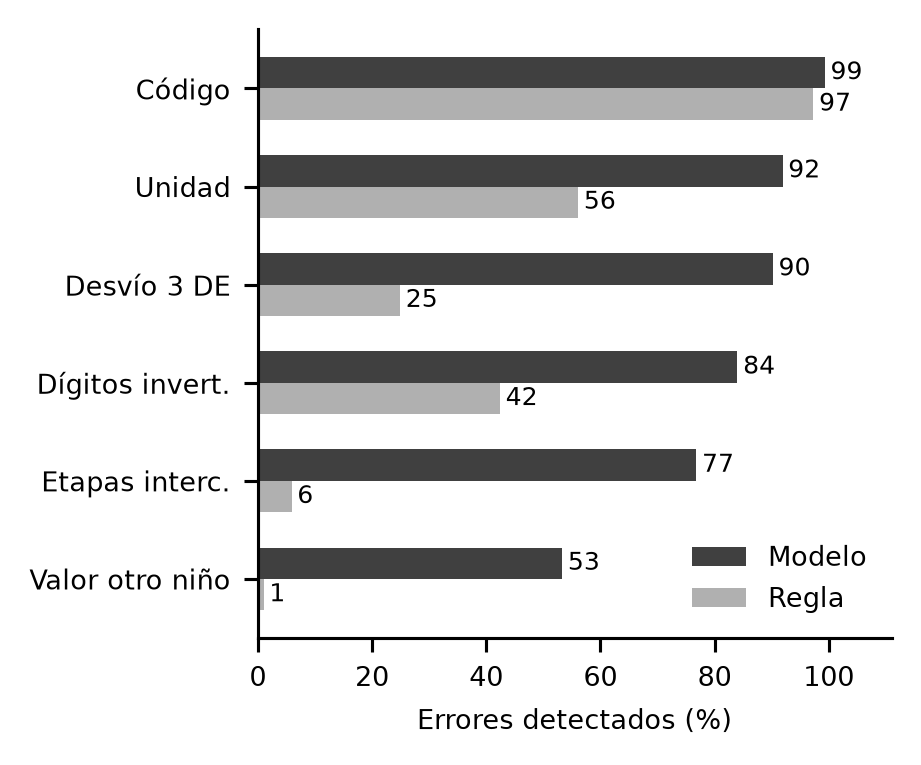
\includegraphics[width=\columnwidth]{figuras/image4.png}
\caption{Porcentaje de errores sintéticos detectados, por categoría: modelo de anomalías en producción (versión 7, $\alpha$ = 0,05) frente a la regla de rangos. Elaboración propia a partir de las métricas registradas en MLflow.}
\label{fig:4}
\end{figure}

\subsection{Evaluación retrospectiva y priorización clínica}
\label{sec:4.3}

Las particiones se describen en la sección~\ref{sec:3.4}; los N de las Tablas~\ref{tab:2} y~\ref{tab:3} son menores que la partición de prueba porque cada desenlace solo incluye a los niños con el resultado ya observado.

Al comenzar el proyecto estudiamos 14 desenlaces relacionados con readmisiones, inasistencias, uso de oxígeno y desarrollo psicomotor. Frente a una referencia sencilla, el modelo obtuvo una AUROC mayor en 13 y empató en uno (Figura~\ref{fig:5} y Tabla~\ref{tab:2}). Un resultado destacado fue la oxigenodependencia a tres meses: AUROC de 0,91 frente a 0,80. No todos los resultados fueron igualmente favorables; algunos desenlaces de inasistencia y readmisión tardía tuvieron discriminación limitada o riesgos sobreestimados.

\begin{figure}[t]
\centering
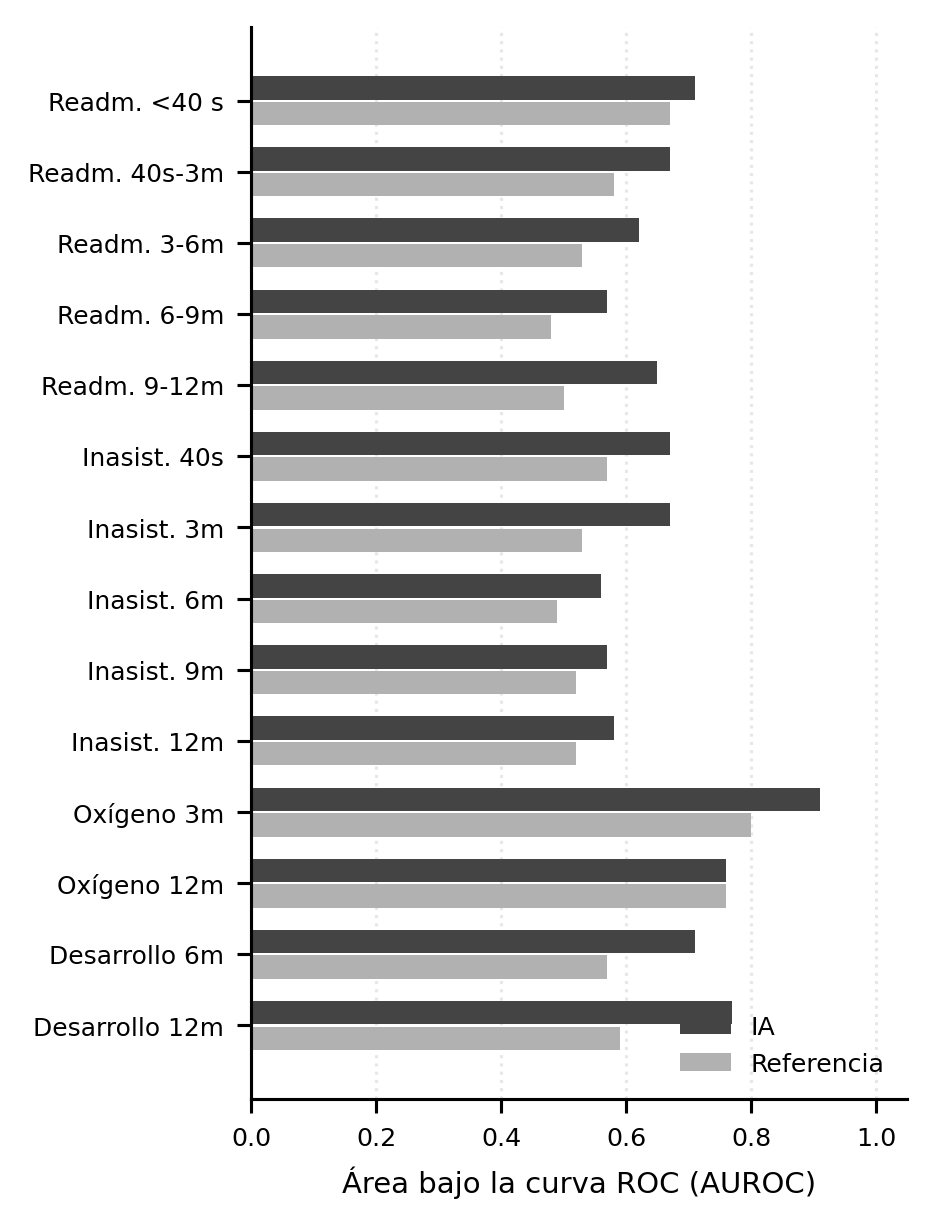
\includegraphics[width=\columnwidth]{figuras/image5.png}
\caption{Comparación de AUROC por desenlace entre el modelo completo y la referencia. Elaboración propia a partir de los resultados retrospectivos.}
\label{fig:5}
\end{figure}

La Tabla~\ref{tab:2} presenta los resultados de la evaluación inicial y el número de niños elegibles para cada desenlace. La relación R/O compara el riesgo medio estimado con la proporción observada; cuando supera 1, el modelo está sobreestimando el riesgo en promedio. Esto ocurrió, por ejemplo, en la readmisión entre 3 y 6 meses, con una relación de 2,96. Aunque el modelo distinguiera mejor a los niños que la referencia, esa diferencia nos recordó que una buena AUROC no garantiza probabilidades bien calibradas \cite{r18,r19}.

\begin{table}[t]
\centering
\caption{Discriminación y relación riesgo/observado por desenlace}
\label{tab:2}
\footnotesize
\setlength{\tabcolsep}{2pt}
\begin{tabular}{@{}lrrrr@{}}
\toprule
\textbf{Desenlace} & \textbf{N} & \textbf{AUC IA} & \textbf{AUC base} & \textbf{R/O} \\
\midrule
Readm. \textless40 s & 6.323 & 0,71 & 0,67 & 1,64 \\
Readm. 40s-3m & 3.886 & 0,67 & 0,58 & 1,39 \\
Readm. 3-6m & 3.385 & 0,62 & 0,53 & 2,96 \\
Readm. 6-9m & 2.615 & 0,57 & 0,48 & 1,59 \\
Readm. 9-12m & 2.295 & 0,65 & 0,50 & 2,01 \\
Inasist. 40s & 2.222 & 0,67 & 0,57 & 0,98 \\
Inasist. 3m & 4.338 & 0,67 & 0,53 & 0,97 \\
Inasist. 6m & 4.660 & 0,56 & 0,49 & 0,90 \\
Inasist. 9m & 3.855 & 0,57 & 0,52 & 0,84 \\
Inasist. 12m & 3.150 & 0,58 & 0,52 & 1,06 \\
Oxígeno 3m & 5.315 & 0,91 & 0,80 & 1,58 \\
Oxígeno 12m & 2.140 & 0,76 & 0,76 & 0,98 \\
Desarrollo 6m & 3.187 & 0,71 & 0,57 & 0,99 \\
Desarrollo 12m & 2.343 & 0,77 & 0,59 & 0,91 \\
\bottomrule
\end{tabular}
\end{table}

Las Figuras~\ref{fig:3}--\ref{fig:5} se elaboraron con los resultados de la evaluación retrospectiva descrita; son gráficas de síntesis preparadas por el equipo.

A partir de las observaciones del experto clínico, decidimos centrar KMCPred en dos desenlaces a los 12 meses EC: talla baja y desarrollo psicomotor bajo. El paquete clínico v8 del 21 de noviembre de 2026 incluye cuatro modelos de talla baja, que hacen estimaciones desde las 40 semanas de edad posmenstrual y los 3, 6 y 9 meses EC, y uno de desarrollo psicomotor, calculado a los 6 meses EC, ver figura~\ref{fig:6}.

\begin{figure}[t]
\centering
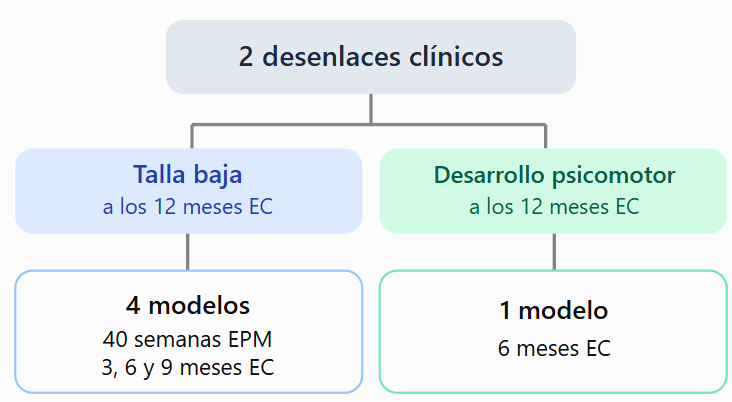
\includegraphics[width=\columnwidth]{figuras/image6.png}
\caption{Relación de modelos y desenlaces abordados. \fuente{Elaboración propia}}
\label{fig:6}
\end{figure}

La Tabla~\ref{tab:3} reúne sus resultados en una evaluación temporal independiente. No mezclamos esas cifras con los 14 desenlaces de la exploración inicial; por eso la referencia de desarrollo psicomotor es 0,59 en la Tabla~\ref{tab:2} y 0,62 en la Tabla~\ref{tab:3}: la primera proviene de la exploración inicial y la segunda, del entrenamiento n.º 15. Además, la categoría «desarrollo psicomotor bajo» se definió para este proyecto y no debe entenderse como diagnóstico clínico.

\begin{table}[t]
\centering
\caption{Resultados de los cinco modelos predictivos asociados a los dos desenlaces clínicos priorizados}
\label{tab:3}
\footnotesize
\setlength{\tabcolsep}{2pt}
\begin{tabular}{@{}p{0.24\columnwidth}p{0.19\columnwidth}p{0.22\columnwidth}p{0.12\columnwidth}p{0.15\columnwidth}@{}}
\toprule
\textbf{Desenlace y corte} & \textbf{N (prev.)} & \textbf{AUROC IA (IC 95\%)} & \textbf{AUROC base} & \textbf{PR-AUC / F1} \\
\midrule
Psicomotor 12m · 6m & 2.343 (4,7\%) & 0,77 (0,72-0,81) & 0,62 & 0,21 / 0,27 \\
Talla baja 12m · 40s & 2.072 (17,6\%) & 0,79 (0,77-0,81) & 0,61 & 0,43 / 0,38 \\
Talla baja 12m · 3m & 2.625 (19,4\%) & 0,86 (0,84-0,87) & 0,60 & 0,61 / 0,46 \\
Talla baja 12m · 6m & 2.420 (19,1\%) & 0,91 (0,89-0,92) & 0,59 & 0,74 / 0,57 \\
Talla baja 12m · 9m & 2.210 (18,9\%) & 0,93 (0,92-0,94) & 0,60 & 0,80 / 0,61 \\
\bottomrule
\end{tabular}
\end{table}

En talla baja encontramos que el desempeño mejora a medida que se dispone de más controles: la AUROC pasó de 0,79 a las 40 semanas a 0,93 a los 9 meses. No obstante, una predicción a los 9 meses deja menos tiempo para actuar que una realizada desde el primer control. A los 6 meses, el modelo alcanzó PR-AUC de 0,74 y F1 de 0,57 para el 10 \% de mayor riesgo; su riesgo promedio estimado (19,5 \%) fue cercano a la frecuencia observada (19,1 \%). Para desarrollo psicomotor, con una prevalencia de 4,7 \%, se obtuvo AUROC de 0,77, precisión de 19,7 \% y F1 de 0,27. Estas cifras muestran potencial, pero también la necesidad de estudiar cuántas alertas podría revisar el equipo clínico.

Al alertar al 10 \% de mayor riesgo, el modelo de talla baja de los 6 meses obtuvo sensibilidad de 43,2 \%, precisión de 82,2 \% y F1 de 0,57. Con información de las 40 semanas, las cifras fueron 29,9 \%, 52,7 \% y 0,38. La comparación ilustra una decisión importante: con más información podemos ganar precisión, pero perdemos parte de la anticipación. Las subcohortes evaluadas tampoco son idénticas, de modo que estas diferencias no demuestran por sí solas un beneficio clínico.

\subsubsection{Matriz de confusión y costos de alertar}
\label{sec:4.3.1}

Como ejemplo del efecto de los umbrales, retomamos el experimento inicial de oxigenodependencia a tres meses. De 5.315 niños, 201 presentaron el desenlace (3,8 \%). Al alertar al 10 \% de mayor riesgo se obtuvieron 143 verdaderos positivos, 389 falsos positivos, 58 falsos negativos y 4.725 verdaderos negativos (Figura~\ref{fig:7}).

\begin{figure}[t]
\centering
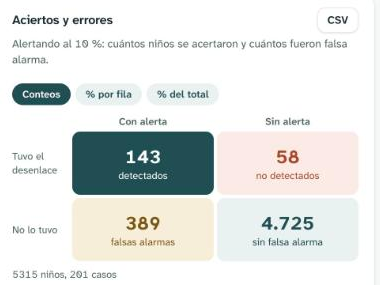
\includegraphics[width=\columnwidth]{figuras/image7.png}
\caption{Matriz de confusión de oxigenodependencia a tres meses al alertar al 10 \% con mayor riesgo (evaluación anterior al paquete clínico v8).}
\label{fig:7}
\end{figure}

Cuando aumentamos la proporción de niños alertados del 5 \% al 20 \%, la sensibilidad pasó del 47,3 \% al 88,1 \%, pero la precisión bajó del 35,7 \% al 16,7 \% (Tabla~\ref{tab:4}). Esto muestra por qué la decisión sobre el umbral debe tomarse con los profesionales: detectar más casos también implica revisar más alertas que finalmente no tendrán el desenlace.

\begin{table}[t]
\centering
\caption{Métricas de oxigenodependencia a tres meses según la proporción alertada (evaluación histórica)}
\label{tab:4}
\footnotesize
\setlength{\tabcolsep}{2pt}
\begin{tabular}{@{}lrrrr@{}}
\toprule
\textbf{Proporción} & \textbf{Sensibilidad} & \textbf{Especificidad} & \textbf{Precisión} & \textbf{F1} \\
\midrule
5 \% & 47,3 \% & 96,7 \% & 35,7 \% & 0,41 \\
10 \% & 71,1 \% & 92,4 \% & 26,9 \% & 0,39 \\
20 \% & 88,1 \% & 82,7 \% & 16,7 \% & 0,28 \\
\bottomrule
\end{tabular}
\end{table}

La Figura~\ref{fig:8} presenta las curvas ROC y precisión--recobrado del modelo de talla baja a los 12 meses EC, utilizando información hasta los 6 meses EC. Su AUROC de 0,91 y PR-AUC de 0,74 reflejan una buena capacidad para diferenciar los casos en la prueba temporal. Aun así, estas curvas no indican por sí solas si el porcentaje de riesgo es acertado; para eso revisamos también la calibración de la Figura~\ref{fig:10}.

\begin{figure}[t]
\centering
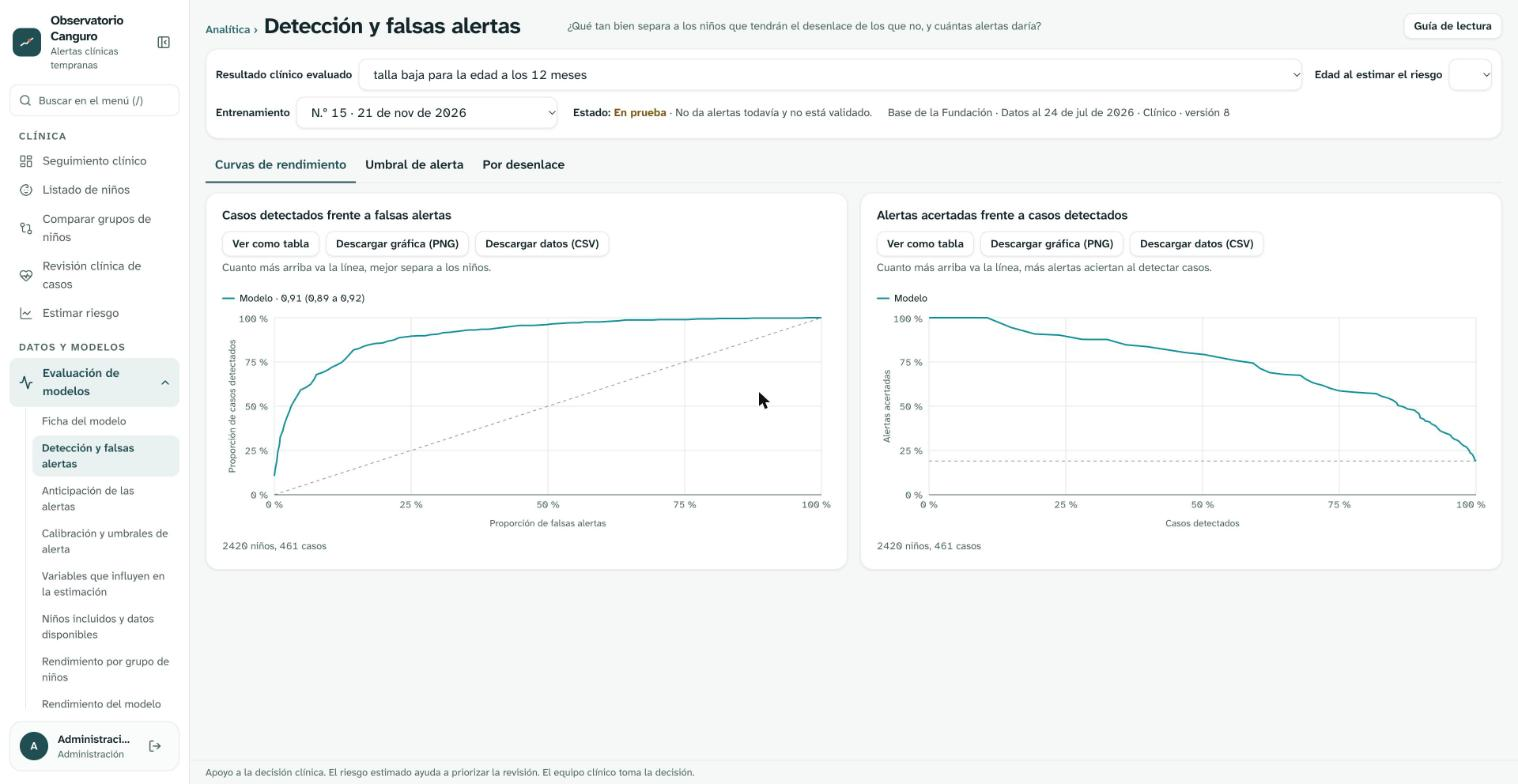
\includegraphics[width=\columnwidth]{figuras/image8.jpg}
\caption{Curvas ROC y precisión--recobrado para talla baja a los 12 meses, estimada a los 6 meses EC}
\label{fig:8}
\end{figure}

\subsection{Crecimiento, denominadores y anticipación}
\label{sec:4.4}

Según los estándares OMS, la proporción de registros por debajo de $-$2 DE fue mayor para talla (18,6--22,4 \%, según la visita) que para peso (10,6--12,0 \%). La Tabla~\ref{tab:5} resume esos resultados iniciales por medición. En la aplicación actual revisamos también el número de niños, para evitar contar varias veces a quienes tienen más de un dato: a las 40 semanas había 24.007 registros de peso, pero correspondían a 20.800 niños. Esta distinción es importante para interpretar cualquier porcentaje clínico.

\begin{table}[t]
\centering
\caption{Porcentaje de registros antropométricos con z inferior a $-$2 DE en el análisis inicial (el recuento por niño de la versión publicada es distinto)}
\label{tab:5}
\footnotesize
\setlength{\tabcolsep}{2pt}
\begin{tabular}{@{}lrrrrr@{}}
\toprule
\textbf{Indicador} & \textbf{40 sem.} & \textbf{3 m} & \textbf{6 m} & \textbf{9 m} & \textbf{12 m} \\
\midrule
Peso & 11,7 & 10,6 & 12,0 & 11,5 & 10,7 \\
Talla & 20,5 & 22,4 & 20,4 & 18,9 & 18,6 \\
P. cefálico & 1,1 & 4,2 & 3,3 & 3,3 & 3,7 \\
\bottomrule
\end{tabular}
\end{table}

\fuente{análisis antropométrico inicial del corte}. Los porcentajes por registro no equivalen necesariamente a prevalencias por niño; la versión publicada corrigió la agregación. Una señal de z \textless{} $-$2 es motivo de vigilancia, no diagnóstico automático.

\subsection{Aplicación, trazabilidad y evidencia operativa}
\label{sec:4.5}

KMCPred se encuentra disponible en \url{https://maia.canbby.com}. Su recorrido permite consultar el seguimiento clínico, explorar grupos mediante filtros, comparar dos cohortes, revisar la ficha de un niño y estimar riesgos. Los apartados técnicos incluyen evaluación de modelos y operación del sistema (Tabla~\ref{tab:6}). La información a la que accede cada persona depende de su perfil: Consulta, Experto clínico, Experto en datos o Administración.

\begin{table}[t]
\centering
\caption{Recorrido funcional de la aplicación}
\label{tab:6}
\footnotesize
\setlength{\tabcolsep}{2pt}
\begin{tabular}{@{}p{0.34\columnwidth}p{0.58\columnwidth}@{}}
\toprule
\textbf{Módulo} & \textbf{Composición} \\
\midrule
Seguimiento clínico & Cohorte, filtros, crecimiento y resultados a 12 m \\
Comparar grupos & Cohortes A/B con criterios, tamaño y gráficos \\
Predicción individual & Caso sintético por visita, riesgo y versión (Fig.~\ref{fig:12}) \\
Evaluación de modelos & Ficha, ROC/PR, calibración e interpretabilidad (Figs.~\ref{fig:8}--\ref{fig:11}) \\
Calidad y operación & Alertas, revisión, administración y configuración \\
\bottomrule
\end{tabular}
\end{table}

La Tabla~\ref{tab:7} muestra los conteos de las matrices de confusión de los cinco modelos del paquete v8 cuando se alerta al 10 \% de mayor riesgo. Son los valores con que se calcularon el F1 de la Tabla~\ref{tab:3} y la sensibilidad y precisión citadas en la sección~\ref{sec:4.3}.

\begin{table}[t]
\centering
\caption{Matrices de confusión de los cinco modelos del paquete v8 al alertar al 10 \% de mayor riesgo (prueba temporal, entrenamiento n.º 15)}
\label{tab:7}
\footnotesize
\setlength{\tabcolsep}{2pt}
\begin{tabular}{@{}lrrrr@{}}
\toprule
\textbf{Modelo · corte} & \textbf{VP} & \textbf{FP} & \textbf{FN} & \textbf{VN} \\
\midrule
Psicomotor 12 m · 6 m EC & 46 & 188 & 63 & 2.046 \\
Talla baja 12 m · 40 sem. & 109 & 98 & 256 & 1.609 \\
Talla baja 12 m · 3 m EC & 179 & 83 & 331 & 2.032 \\
Talla baja 12 m · 6 m EC & 199 & 43 & 262 & 1.916 \\
Talla baja 12 m · 9 m EC & 196 & 25 & 221 & 1.768 \\
\bottomrule
\end{tabular}
\end{table}

El servidor utilizado dispone de un procesador AMD Ryzen 9 7900X, una GPU RTX 5060 Ti y 30,45 GiB de RAM. En 17 predicciones individuales realizadas desde el navegador el 21 de noviembre de 2026, el tiempo mediano fue 2,54 s y el percentil 95 alcanzó 2,61 s. Entrenar los cinco modelos clínicos v8 tomó aproximadamente tres minutos. Son resultados de esas pruebas puntuales; no permiten afirmar cómo respondería el sistema con muchos usuarios simultáneos.

La Figura~\ref{fig:9} recoge la ficha del modelo de talla baja a los 12 meses, estimada a los 6 meses EC. En la plataforma este modelo aparece «En prueba», por lo que sus resultados deben entenderse como parte de la evaluación y no como una herramienta clínica ya validada. Al comparar grupos A/B, también es importante mostrar claramente los filtros utilizados, los tamaños de ambos grupos y los datos disponibles.

\begin{figure}[t]
\centering
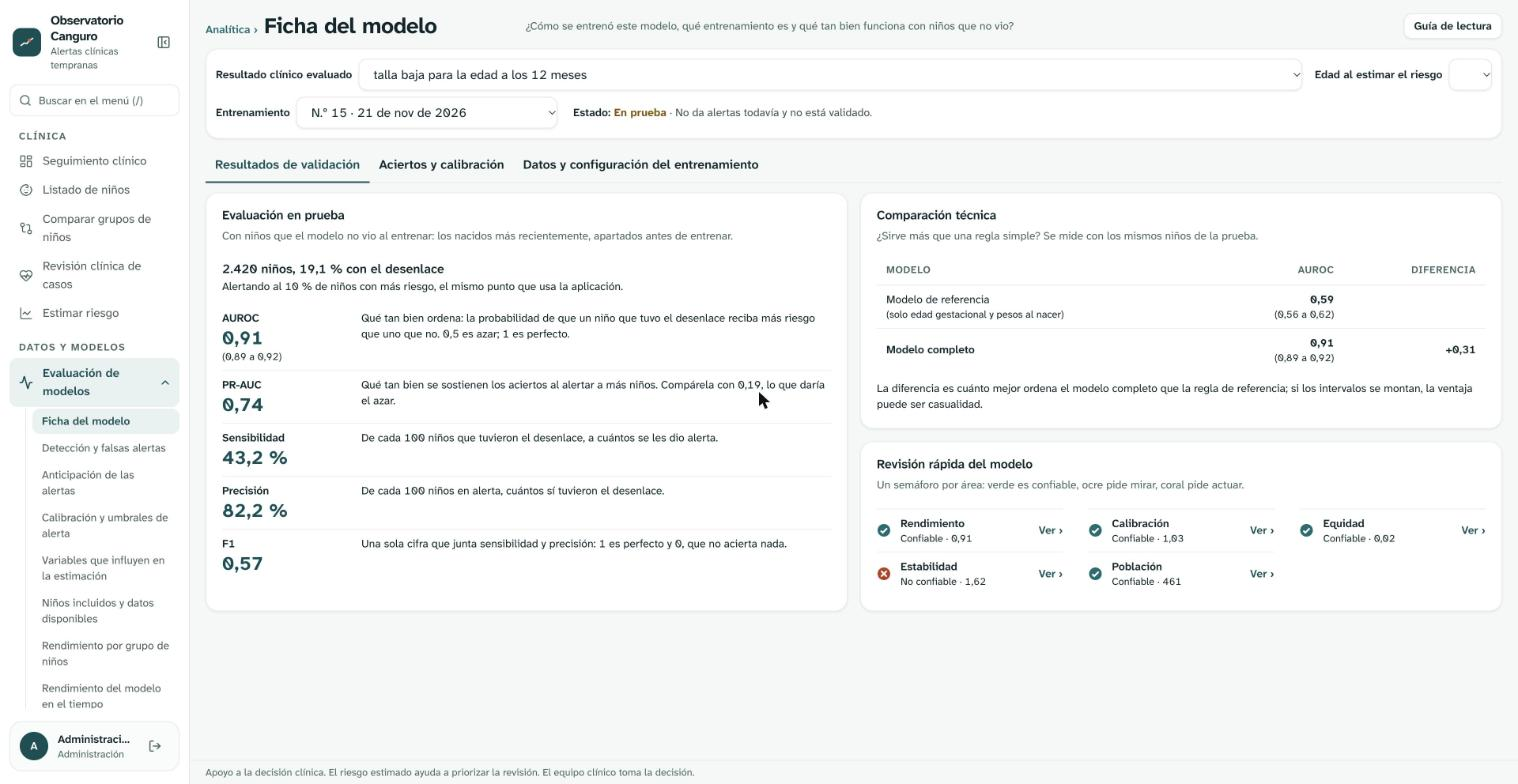
\includegraphics[width=\columnwidth]{figuras/image9.jpg}
\caption{Ficha del modelo: talla baja a 12 meses estimada a 6 meses EC, entrenamiento n.º 15 y paquete v8.}
\label{fig:9}
\end{figure}

La Figura~\ref{fig:10} compara, por grupos de riesgo, las probabilidades calculadas para talla baja a los 12 meses desde los 6 meses EC con los resultados observados. El promedio predicho fue 19,5 \% y el observado 19,1 \% (relación 1,03; error medio de calibración 0,026; Brier 0,087). Es una señal favorable dentro de esta evaluación retrospectiva, pero no reemplaza la validación prospectiva ni garantiza que el modelo funcione igual en todos los subgrupos.

\begin{figure}[t]
\centering
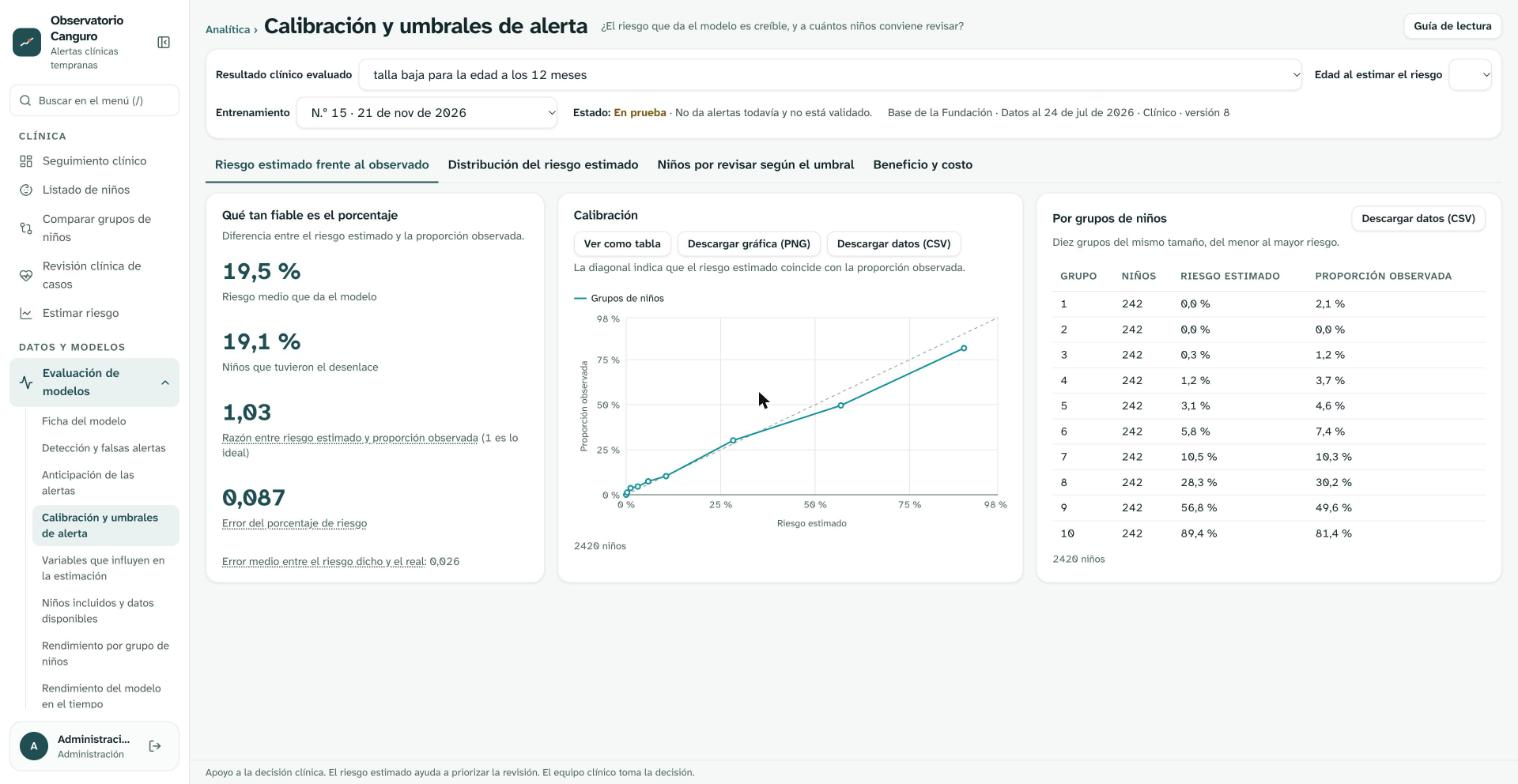
\includegraphics[width=\columnwidth]{figuras/image10.jpg}
\caption{Calibración por deciles de la probabilidad de talla baja a 12 meses calculada a los 6 meses EC (paquete v8).}
\label{fig:10}
\end{figure}

La Figura~\ref{fig:11} presenta las variables con mayor importancia global en el modelo de desarrollo psicomotor bajo, medida como la ganancia que aporta cada variable en LightGBM. Estas importancias muestran patrones aprendidos, no causas clínicas. TreeSHAP se usa en la explicación individual de cada niño. Algunas variables aparecen con su código del diccionario del Observatorio Canguro, tal como las muestra la plataforma.

\begin{figure}[t]
\centering
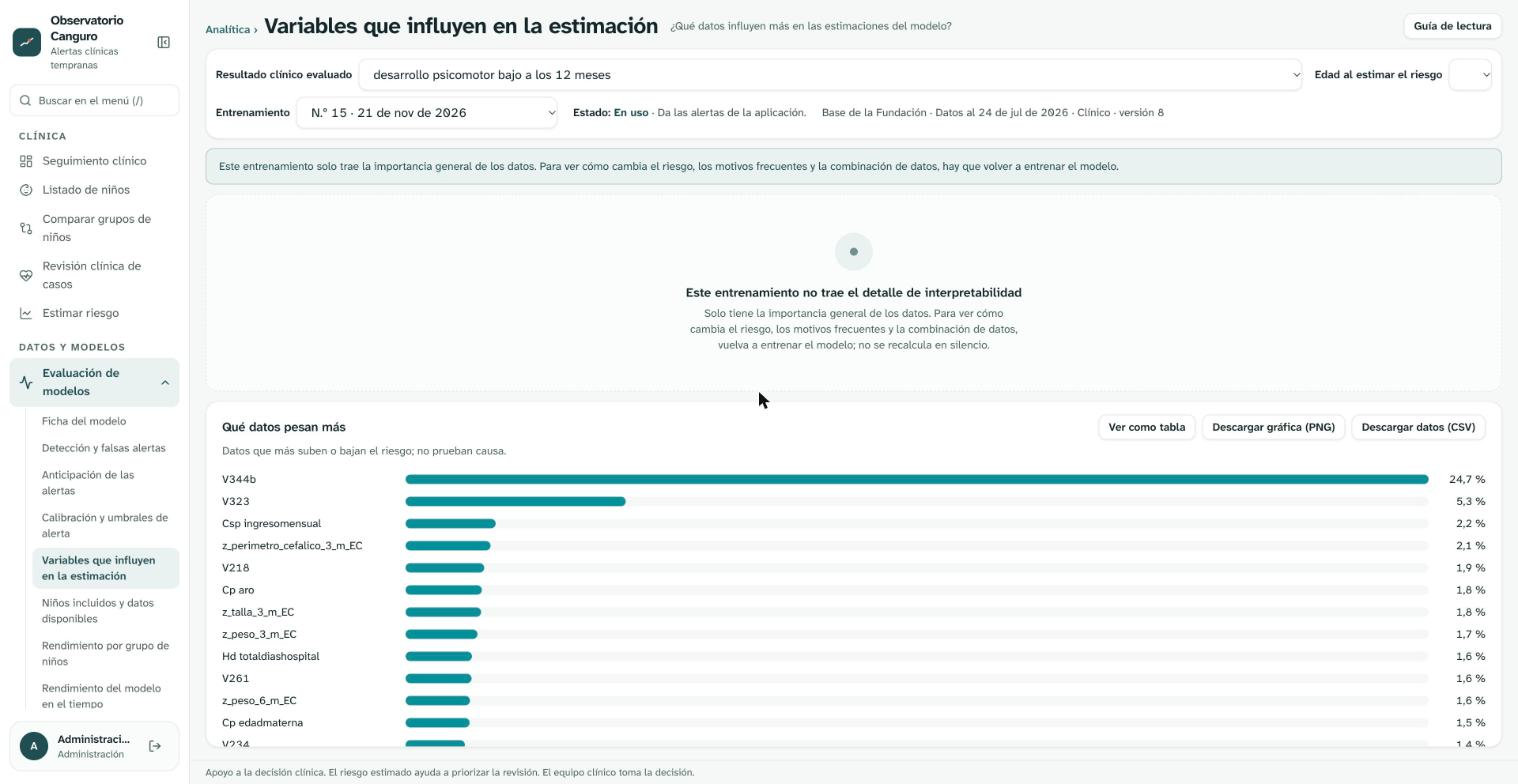
\includegraphics[width=\columnwidth]{figuras/image11.jpg}
\caption{Importancia global de variables (ganancia de LightGBM) del desenlace desarrollo psicomotor bajo a los 12 meses; captura del paquete activo. Las variables se muestran con su código del diccionario.}
\label{fig:11}
\end{figure}

La Figura~\ref{fig:12} presenta un niño simulado cuyo riesgo de talla baja a los 12 meses se consulta desde las 40 semanas y los 3, 6 y 9 meses EC; cada estimación debe usar solo datos disponibles hasta su corte.

\begin{figure}[t]
\centering
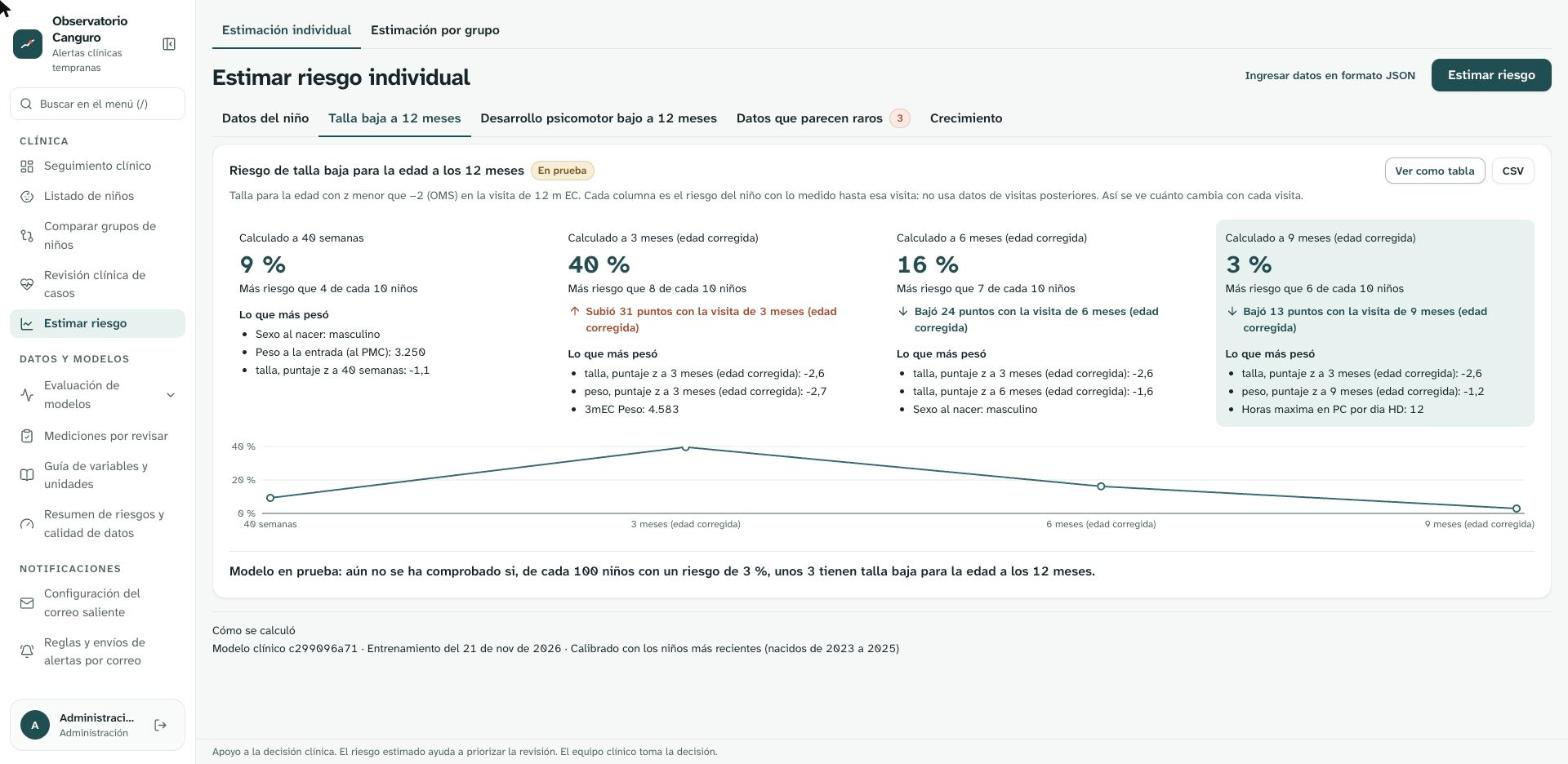
\includegraphics[width=\columnwidth]{figuras/image12.jpg}
\caption{Estimación de talla baja a 12 meses para un niño simulado desde distintas visitas; cada cálculo usa solo información previa a su corte.}
\label{fig:12}
\end{figure}
